\resetfigpath{5-software}

\chapter{Annotation tools}
In the frame of this thesis, a flexible annotation software was developed that supports both the traditional mouse input as well as an interface to connect an eye-gaze tracker.
Also, a web interface was designed and implemented that allows a user to upload a sequence annotated using the above software, and obtain a pixel-wise segmentation.
We now describe both contributions.

\section{Sequence annotation tool}
\label{sec:anna}

We developed an annotation software that allows a user to generate point-wise coordinates according to the given protocol.

\begin{enumerate}
  \item[-]{Provide as input a volume/video. These can be either DICOM \cite{dicom}, or video files.}
  \item[-]{Optional: Set the framerate at which the sequence will play (right knob on Fig. \ref{fig:anna}).}
  \item[-]{Optional: Connect the software to the eye-gaze tracker server. The tracker will then act as a secondary mouse.}
  \item[-]{Hit the play button. The sequence unfolds.}
  \item[-]{Give point annotations:}
    \begin{itemize}
      \item[-]{When using mouse: Simply click on the desired region.}
      \item[-]{When using gaze-tracker: Place gaze on region and use right button (Fig. \ref{fig:anna}) to activate the recording of locations.}
    \end{itemize}
  \item[-]{Save locations in \gls{csv} file.}
\end{enumerate}

\begin{figure}[!htpb]
  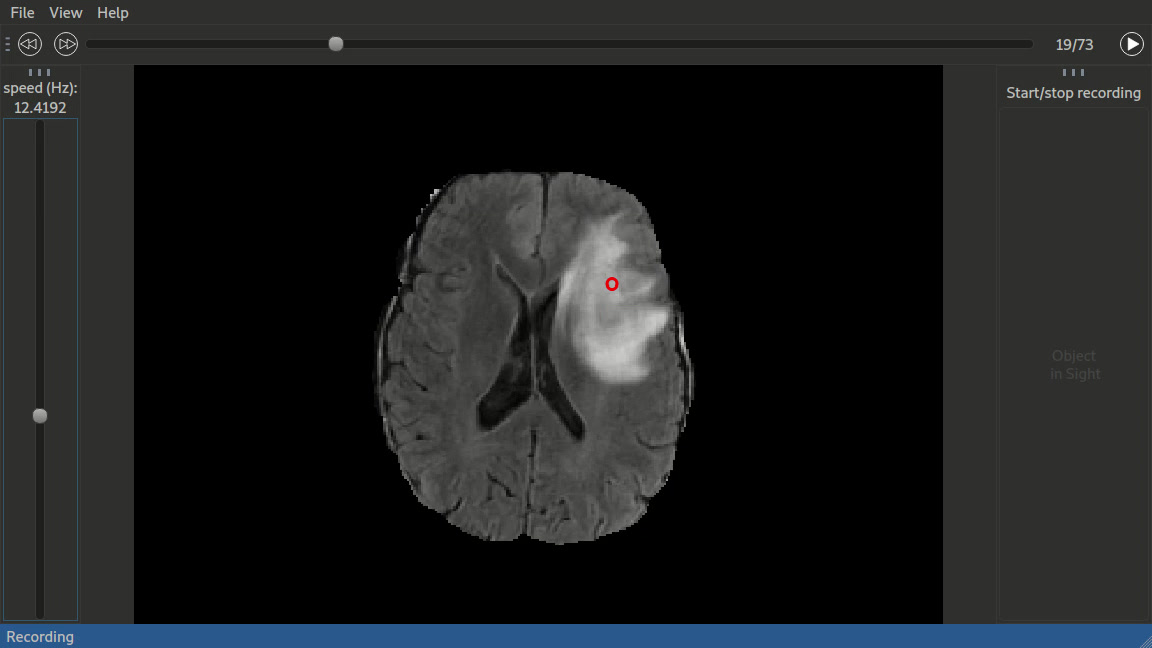
\includegraphics[width=0.99\textwidth]{anna0.png}
  \caption{Screenshot of annotation tool. }
  \label{fig:anna}
\end{figure}

\subsection{Implementation}
The annotation software is intended to be cross-platform and be compatible with a variety of input formats.
Second, as our early experiments relied on an eye-gaze tracker, our software needed to be compatible with the proprietary backend given by the manufacturer.
Third, a simple \gls{gui} was needed to display images and allow the user to select his favorite modality of annotation.
The latter requirements drove our choice towards the Qt5 framework \cite{eng16}, which relies on C++ and provides convenient widgets out of the box.
Our software supports allows to annotate using a mouse and an eye-gaze tracker \cite{eyetribe}.
As platform, it supports the Linux, MacOS and Windows operating systems.
We provide the source code at \href{https://github.com/aimi-lab/Anna}.

\section{Web platform}
The segmentation methods presented in the next chapters require important computational resources, namely a GPU to train deep networks.
We therefore provide a way for users to upload their data along with the corresponding 2D locations to a server that will perform the necessary computations remotely and send back segmentation results.
Concretely, we develop a web interface that provides:

\begin{itemize}
  \item[-]{Links to download the annotation software (Sec. \ref{sec:anna}).}
  \item[-]{A login mechanism that provides us with a contact e-mail address.}
  \item[-]{An upload form where the user drops his sequence along with the 2D locations}
\end{itemize}

Once the data has been uploaded, a task object is created and queued until computational resources are available.
After completion, the user is warned that he can download his segmentations via a URL.

\begin{figure}[!htpb]
  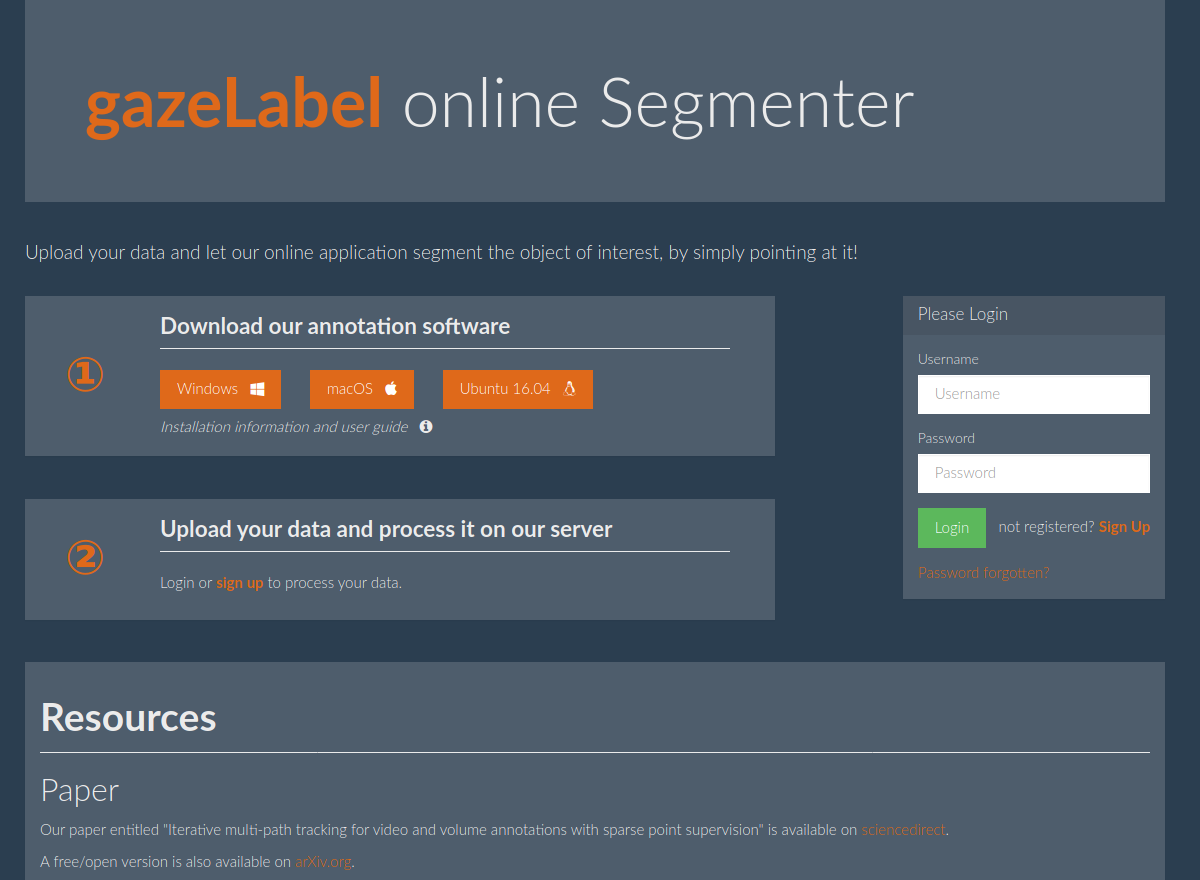
\includegraphics[width=0.99\textwidth]{gazelabel.png}
  \caption{Screenshot of our web platform. Home page.}
  \label{fig:anna}
\end{figure}

\subsection{Implementation}
The frontend, which generates the web pages uses the \href{https://webpack.js.org}{Webpack} bundler.
The backend is based on the \href{https://www.djangoproject.com/}{Django} framework, which handles different applications, namely the forms (login, data upload), the job queue, and the database.

\begin{figure}[!htpb]
  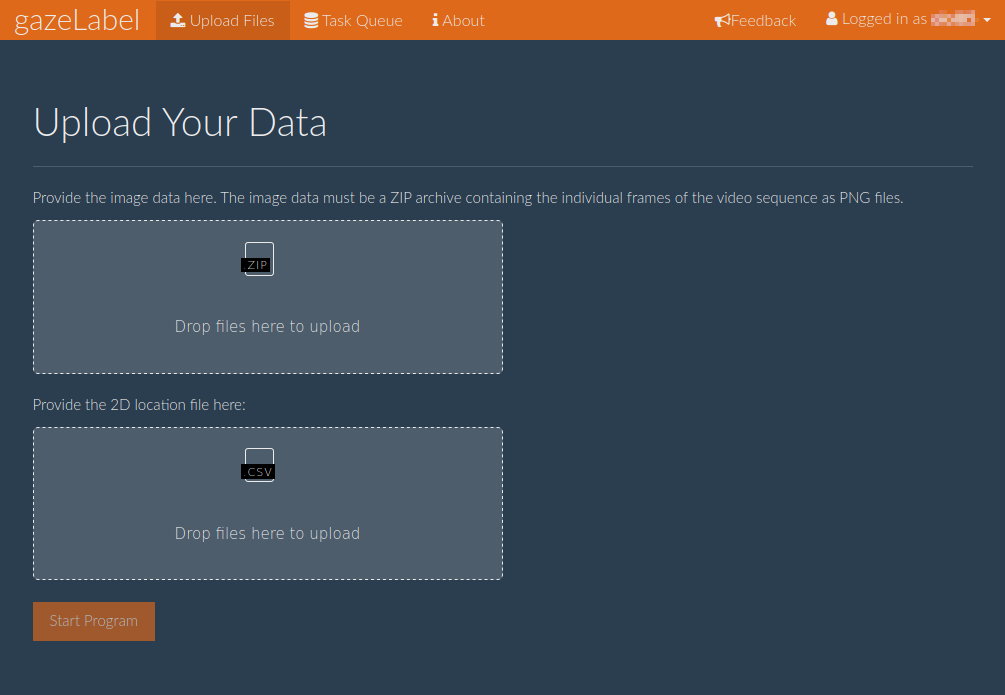
\includegraphics[width=0.99\textwidth]{gazelabel_upload.png}
  \caption{Screenshot of our web platform, where the user can upload a sequence and its corresponding annotations. The task queue panel shows the state of the submitted tasks.}
  \label{fig:anna_upload}
\end{figure}

%%% Local Variables:
%%% mode: latex
%%% TeX-master: "../../main"
%%% End:
